\documentclass[9pt,twocolumn,twoside]{pnas-report}

\usepackage{todonotes}

\setuptodonotes{inline,size=\small,color=blue!40}

\templatetype{pnasresearcharticle}

\usepackage{numprint}


\titlespacing\section{0pt}{2pt plus 0pt minus 2pt}{0pt plus 0pt}

\titlespacing\subsection{10pt}{2pt plus 0pt minus 2pt}{3pt plus 00pt}


% set figures directory to be ./figures
\graphicspath{{./figures/}}

\title{Vulnerability Reach in Package Ecosystems}

\author[a]{Žiga Trček}
\author[a]{Matej Urbas}
\author[a]{Jan Vasiljević}

\affil[a]{University of Ljubljana, Faculty of Computer and Information Science, Ve\v{c}na pot 113, SI-1000 Ljubljana, Slovenia}

\leadauthor{Jan Vasiljević, Žiga Trček, Matej Urbas}


\begin{abstract}
	The rapid integration of open-source packages into software development introduces significant security challenges. 
	This study investigates these risks in light of a recent incident involving OpenSSH, where a malicious actor exploited a transitive dependency. 
	Focusing on three major package ecosystems—PyPI, npm, and crates.io—we examine their dependency networks to assess vulnerability to malicious packages. 
	We analyze how vulnerabilities propagate through these networks and identify the communities within each ecosystem that are most susceptible to attacks. 
	Our findings demonstrate the need for minimizing dependencies to enhance security, particularly in production environments, where reduced dependencies mitigate risk exposure.
\end{abstract}
	
\dates{The manuscript was compiled on \today}
\doi{\href{https://ucilnica.fri.uni-lj.si/course/view.php?id=183}{Introduction to Network Analysis} 2023/24}

\begin{document}

\maketitle
\thispagestyle{firststyle}
\ifthenelse{\boolean{shortarticle}}{\ifthenelse{\boolean{singlecolumn}}{\abscontentformatted}{\abscontent}}{}

\dropcap{T}he date is March 28, 2024. A principal software engineer at Microsoft notices an unusual delay in his login attempts, timing at approximately 500ms—significantly longer than usual by his standards.
This prompts an investigation into higher-than-normal CPU usage, during which he observes anomalous behavior in the SSH daemon process.
This unexpected discovery leads to the identification of a vulnerability in the XZ Utils library utilized by OpenSSH.
The breach, orchestrated by a malicious actor through a combination of social engineering, code injection, and obfuscation, was set into motion over several years.
Interestingly, the core code of OpenSSH remained untouched; instead, a transitive dependency was exploited.
Had this vulnerability remained undetected, it could have potentially compromised a vast number of servers relying on OpenSSH, embedding a remote code execution backdoor.


Like the exploitation of the XZ Utils library, other open-source software packages and libraries are also vulnerable to malicious attacks.
The development of software inherently involves placing trust in the authors of utilized libraries, who are often individual hobbyists or small teams with limited resources.
The potential for significant damage is large if a malicious actor targets a lesser-maintained package that, while small, is widely used—either directly or as a transitive dependency in other software projects.
The incident involving the left-pad package, which was removed from npm and consequently led to the failure of numerous dependent packages, serves as a reminder of the inherent fragility within the open-source ecosystem.

In this project, we look at three different package ecosystems: PyPI \cite{pypi}, npm \cite{NPM}, and crates.io \cite{crates}, which are package repositories for Python, JavaScript, and Rust, respectively.
We aim to investigate the security of these ecosystems by conceptualizing them as networks and integrating external vulnerability data in our analysis.
Our primary goal and contribution is to understand how vulnerabilities propagate through these networks and identify the communities within each ecosystem that are most susceptible to attacks.
While a lot of research has been on the security of dependency networks through network analysis,
we found a lack of research on this kind of analysis.
Our report can be summarized in \ref{fig:topdown}.


\begin{figure}
	\centering
	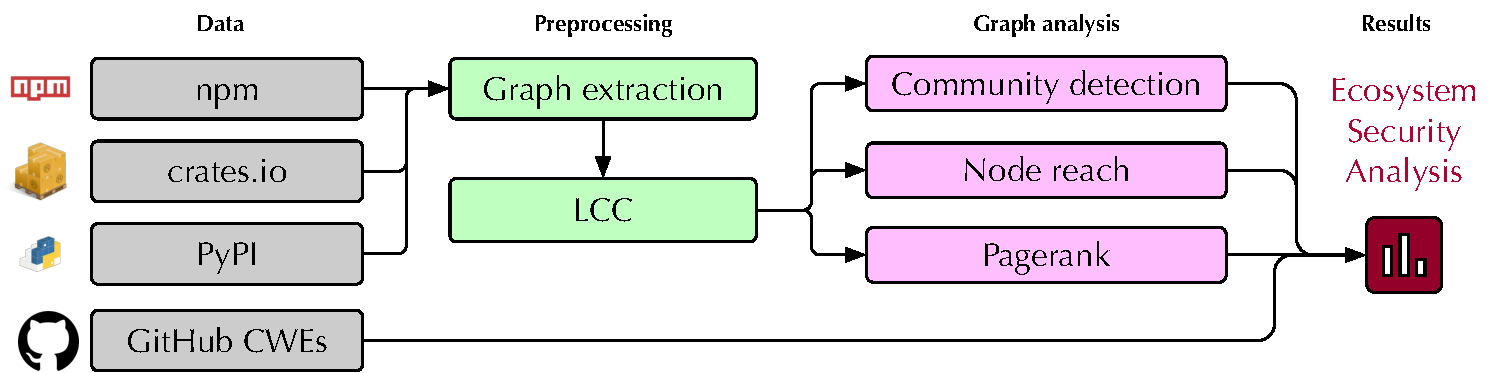
\includegraphics[width=1\linewidth]{topdown.pdf}
	\caption{Mandatory informative illustration highlighting main contributions.}
	\label{fig:topdown}
\end{figure}
\section*{Related Work}

The robustness of dependency networks has been extensively studied in various contexts. \cite{hafner2021robustness} focused on the npm package dependency network, highlighting its vulnerability to targeted attacks on crucial nodes that, despite being large and well-maintained, significantly impact the network due to their numerous dependencies. The study also notes a trend towards increased robustness as the number of dependencies decreases over time.

\cite{decan2018evolution} provided a comparative analysis of dependency networks across seven package ecosystems, including Cargo, CPAN, CRAN, npm, NuGet, Packagist, and RubyGems. Their work introduced metrics to evaluate growth, changeability, reusability, and fragility, uncovering that while these ecosystems continue to expand, a small number of packages disproportionately influence most updates and dependencies. This study also warned of the risks posed by transitive dependencies on unmaintained or obsolete packages, which can severely affect the security and maintainability of an ecosystem.

\cite{tsakpinis2024accessibility} studied the accessibility of GitHub repositories for npm and PyPI libraries, revealing that a significant portion of libraries lacked valid repository URLs— a critical factor for effective vulnerability monitoring and codebase maintenance.

Community detection has been proposed as a useful method for enhancing network security analysis. Identifying closely connected package groups can reveal potential vulnerabilities and dependencies that could be exploited by attackers, as discussed in \cite{hafner2021robustness} and \cite{tsakpinis2024accessibility}. \cite{korkmazrpackages} further explored the dependency graph of R packages, finding a strong correlation between centrality measures and the popularity of packages, as measured by downloads and citations. The study also highlighted the positive influence of package attributes like the number of authors and commits.

Research on security vulnerabilities has significantly evolved. \cite{decan2018vulnerabilities} analyzed around 400 security reports from the npm network, illustrating the lengthy process from vulnerability discovery to public disclosure and eventual resolution. Similarly, \cite{shahzad2012} examined the life cycles of vulnerabilities in a broad dataset, finding comparable durations.

\cite{HANIF2021103009} proposed and evaluated novel machine learning approaches for predicting vulnerabilities in open-source software, achieving high accuracy even for complex vulnerabilities. \cite{hejderup2018} and \cite{hejderup2022prazi} shifted focus from traditional dependency graphs to call graphs for detecting software dependencies, which helped in the preliminary evaluation of security issues and their broader impact. Their findings suggest that many dependencies in Cargo packages are unnecessary, potentially introducing unneeded vulnerabilities.

\cite{ruohonen2021} conducted a static analysis of approximately \numprint{200000} PyPI packages and discovered that nearly half contained at least one security vulnerability, highlighting the persistent security challenges in open-source software.


\section*{Results}
We analysed three popular programming languages' ecosystems: npm , Crates.io  and PyPI .
Basic stats of each ecosystem's dependency network are shown in Table \ref{tab:basic_stats}.
NPM dependency network is analysed twice, once with combined production and development dependencies, and once with only production dependencies.

\begin{table}[h]\centering%
	\caption{Original dependency networks for all three ecosystems.}
	\begin{tabular}{l|ccccc}
		ecosystem  & $n$       & $m$        & $\langle k\rangle$ & $\langle C\rangle$ & \#CC     \\\hline
		npm        & $2425767$ & $23006281$ & $19$               & $0.18$             & $561569$ \\
		npm (prod) & $2424918$ & $7920337$  & $7$                & $0.06$             & $870151$ \\
		PyPI       & $532386$  & $1649201$  & $6$                & $0.11$             & $179304$ \\
		Crates.io  & $145269$  & $830337$   & $11$               & $0.23$             & $25179$  \\
	\end{tabular}
	\label{tab:basic_stats}
\end{table}

For the rest of our analysis, we only considered the largest weakly connected components.
Statistics of these networks are shown in Table \ref{tab:lcc_stats}.

\begin{table}[h]\centering%
	\caption{Largest connected components for all three ecosystems.}
	\begin{tabular}{l|ccccc}
		ecosystem  & $n$       & $m$        & $\langle k\rangle$ & $\langle C\rangle$ & \% nodes \\\hline
		npm        & $1845838$ & $22979692$ & $24$               & $0.23$             & $76$     \\
		npm (prod) & $1518107$ & $7871828$  & $10$               & $0.10$             & $62$     \\
		PyPI       & $349793$  & $1645588$  & $9$                & $0.17$             & $66$     \\
		Crates.io  & $119461$  & $829615$   & $13$               & $0.28$             & $82$     \\
	\end{tabular}
	\label{tab:lcc_stats}
\end{table}

\subsection*{Vulnerabilities per ecosystem}

By enumerating over vulnerabilities from the GitHub's advisory database we examined the reach of every listed vulnerability.
The vulnerabilities were analysed as if they all occured on the most recent package dependency graphs as we didn't have the required graph history snapshots.
The reach is defined by the size of the affected package's in-component - all the packages that directly or indirectly depend on the affected package.
To get a measure, which is proportional to the graph size and package importance, we summed up the page rank scores from the affected component.
The reach measure for every vulnerability for these ecosystems is shown in Figure \ref{fig:reach}.

\begin{figure}[t]\centering%
	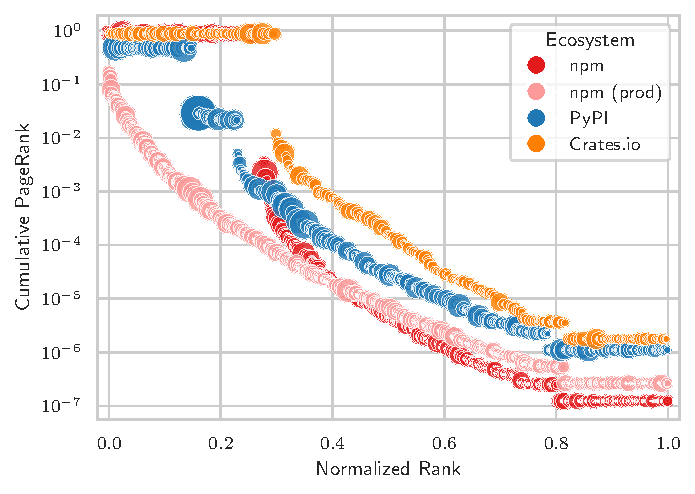
\includegraphics[width=\linewidth]{vuln_pagerank}
	\caption{Vulnerabilities and their reach. Each dot represents a single vulnerability. Dot size represents the vulnerability severity according to CVSS.  }
	\label{fig:reach}
\end{figure}

Crates.io and npm ecosystems are the most vulnerable.
Around 30\% of all vulnerabilities could reach almost every package (~95\% of all).
PyPI is a bit less interwined, with \textit{only} 69\% of packages being affected by the largest vulnerability.
It's also interesting to observe the sudden jumps in the lines.
There appears to be a tipping point between 1\% and 10\% accumulated page rank at which point the entire graph gets infected.
If we exclude all development dependencies from the npm network, we notice a very high decrease in the percentage of affeceted packages.
The npm production network consists of around 3 times less edges than the network which also includes development dependencies.
This might correlate to 3 times the reduction in affected packages.
This also shows that developers are much more exposed than production environments, which keep their dependencies to a minimum.
Vulnerabilities with biggest reach for every ecosystem are listed in Table \ref{tab:highest_reach}.

\begin{table}[h]\centering%
	\caption{Biggest reach vulnerability.}
	\begin{tabular}{l|ccc}
		ecosystem  & package   & \% packages affected & affected pagerant \\\hline
		npm        & lodash    & $93$                 & $0.88$            \\
		npm (prod) & ms        & $\mathbf{30}$        & $\mathbf{0.18}$   \\
		PyPI       & pyOpenSSL & $69$                 & $0.54$            \\
		Crates.io  & shlex     & $95$                 & $0.88$            \\
	\end{tabular}
	\label{tab:highest_reach}
\end{table}

\subsection*{Vulnerabilities per community}
Using the Leiden community detection we extracted communities from dependency networks and analysed top 5 communities with the higest number of packages listed in GitHub's advisory database.
By examining the packages inside these communities we determined the community's general use case.
Due to the randomness, we ran the Leiden community detection multiple times and aggregated the results.

\subsubsection*{Crates.io}
Leiden found 100 communities. There are 472 crates that were once malicious. Communities with the most malicious packages are listed in Table \ref{tab:cargo_comms}.
\begin{table}[h]\centering%
	\caption{Cargo.io affected communities.}
	\begin{tabular}{l|cccc}
		usecase       & \#vulns & packages & \% of all vulns & \% infected \\\hline
		cryptography  & 84      & 11975    & 18              & 0.7         \\
		logging       & 82      & 24868    & 17              & 0.3         \\
		serilization  & 80      & 22882    & 17              & 0.3         \\
		WASM          & 40      & 10044    & 8               & 0.4         \\
		crossplatform & 40      & 8629     & 8               & 0.5         \\
	\end{tabular}
	\label{tab:cargo_comms}
\end{table}
\subsubsection*{PyPI}
Leiden found 216 communities. There are 909 packages that were once malicious. Communities with the most malicious packages are listed in Table \ref{tab:pypi_comms}.
\begin{table}[h]\centering%
	\caption{PyPI affected communities.}
	\begin{tabular}{l|cccc}
		usecase      & \#vulns & packages & \% of all vulns & \% infected \\\hline
		networking   & 273     & 58827    & 30              & 0.5         \\
		data storage & 90      & 22253    & 10              & 0.4         \\
		testing      & 69      & 35476    & 8               & 0.2         \\
		django       & 69      & 13206    & 8               & 0.5         \\
		scraping     & 63      & 47490    & 7               & 0.1         \\
	\end{tabular}
	\label{tab:pypi_comms}
\end{table}

\subsubsection*{npm}
Leiden found 1611 communities. There are 2482 packages that were once malicious. Communities with the most malicious packages are listed in Table \ref{tab:npm_comms}.
\begin{table}[h]\centering%
	\caption{npm affected communities.}
	\begin{tabular}{l|cccc}
		usecase      & \#vulns & packages & \% of all vulns & \% infected \\\hline
		networking   & 582     & 284746   & 23              & 0.2         \\
		command line & 392     & 264426   & 16              & 0.1         \\
		utility      & 213     & 78199    & 9               & 0.3         \\
		react        & 123     & 195990   & 5               & 0.1         \\
		vue          & 97      & 144181   & 4               & 0.1         \\
	\end{tabular}
	\label{tab:npm_comms}
\end{table}

\section*{Conclusion}

In this project, we analyzed the impact of malicious packages on the package managers of three programming languages: Rust's Crates.io, Python's PyPI, and JavaScript's npm.
By examining vulnerabilities listed in GitHub's advisory database over the last eight years, we assessed their influence on these ecosystems.

Our findings highlight that malicious code can significantly affect the vast majority of the JavaScript and Rust ecosystems.
Python's ecosystem, with its less interconnected package structure, shows somewhat better resistance to such threats.
We observed that the most effective protection against malicious packages is to limit dependencies.
For example, npm's production-only dependency network, which excludes development dependencies, has three times fewer connections and only 20\% fewer packages than the full network, effectively reducing the spread of malicious code across more than 30\% of the network.

Each ecosystem has distinct communities that are more vulnerable to attacks.
Rust, being a low-level, high-performance language, is primarily composed of packages that perform fundamental operations like serialization and logging, and it offers strong cross-platform support.
Python's most affected communities highlight its strengths in networking, data scraping, and data manipulation.
The vulnerabilities in npm illustrate JavaScript's prevalent use in web development, particularly with frameworks such as React and Vue.

We had additional research ideas but were limited by data availability.
We aimed to rank malicious packages by their direct and indirect download counts, hypothesizing that the most hazardous packages would have low direct but high indirect downloads.
However, obtaining this data proved challenging due to the dynamic nature of package dependencies and semantic versioning.

\small

\section*{Methods}

\subsubsection*{Data Acquisition} The data for \texttt{crates.io} was acquired from their official website, where daily data dumps are available.
For \texttt{npm}, we initially attempted to follow the official guide on their website to clone the CouchDB database.
However, this method proved to be outdated and non-functional.
Consequently, we utilized data from \cite{npmdata}, which provides a weekly data dump of all npm dependencies.
The entire dataset was 200GB in size and packaged in a PostgreSQL database.
For \texttt{PyPI}, we had to manually scrape the data, as there is no official data dump available.

\subsection*{Data Preprocessing} From the data we acquired, we extracted package names, dependencies, and download counts. We then constructed a simple directed graph where nodes represent packages and edges represent dependencies. The edge direction is from the dependent package to the dependency. Graphs were then reduced to the largest connected component and exported in the \texttt{GraphML} format for further analysis.

\subsection*{\texttt{igraph}} Instead of relying on \texttt{networkx} for network analysis, we used the \texttt{igraph} library \cite{igraph}.
Using \texttt{networkx}, even a simple import of the \texttt{npm} dataset took around 300 seconds.
Additionally, every other operation was significantly slower compared to \texttt{igraph}.

\subsection*{Reach Measure} This measure indicates the potential danger of a vulnerability within a specific package.
The in-component of a malicious package comprises all packages that directly or indirectly depend on it.
If any of these packages are installed, they also install the malicious package.
However, the relative size of the in-component alone does not reflect the significance of the affected packages.
By summing the PageRanks of all packages within the in-component, we obtain a score ranging from 0 to 1, which incorporates the importance of the affected packages.


\subsection*{Community Detection} For community detection, we used the \texttt{leiden} algorithm, which is an efficient method for uncovering community structures in large networks.
The algorithm optimizes the modularity function $ Q $ as $
	Q = \frac{1}{2m} \sum_{ij} \left[ A_{ij} - \frac{k_i k_j}{2m} \right] \delta(c_i, c_j)
$
where \( A_{ij} \) is the weight of the edge between nodes \( i \) and \( j \), \( k_i \) and \( k_j \) are the degrees of nodes \( i \) and \( j \), \( m \) is the total weight of all edges in the graph, and \( \delta(c_i, c_j) \) is the Kronecker delta which is 1 if nodes \( i \) and \( j \) belong to the same community and 0 otherwise.

\normalsize


\bibliography{bibliography}

\end{document}
